% This is a general template file for the LaTeX package SVJour3
% for Springer journals. Original by Springer Heidelberg, 2010/09/16
%
% Use it as the basis for your article. Delete % signs as needed.
%
% This template includes a few options for different layouts and
% content for various journals. Please consult a previous issue of
% your journal as needed.
%
\RequirePackage{fix-cm}
\RequirePackage{amsmath}
%
%\documentclass{svjour3}                     % onecolumn (standard format)
%\documentclass[smallcondensed]{svjour3}     % onecolumn (ditto)
\documentclass[smallextended]{svjour3}       % onecolumn (second format)
%\documentclass[twocolumn]{svjour3}          % twocolumn
%
\smartqed  % flush right qed marks, e.g. at end of proof
%
\usepackage{graphicx}
\usepackage{mathtools}
\usepackage{amsfonts}
%
% insert here the call for the packages your document requires
%\usepackage{mathptmx}      % use Times fonts if available on your TeX system
%\usepackage{latexsym}
% etc.
%
% please place your own definitions here and don't use \def but
% \newcommand{}{}
%
% Insert the name of "your journal" with
% \journalname{myjournal}
%

\newtheorem{prop}{Proposition}
\newtheorem{defn}{Definition}
\providecommand{\HickernellFJ}{Hickernell}
\newcommand{\bm}[1]{\boldsymbol{#1}}
\newcommand{\mSigma}{\mathsf{\Sigma}}
\newcommand{\mB}{\mathsf{B}}
\newcommand{\smallocite}[1]{{\small\ocite{#1}}}
\newcommand{\dif}[1]{\text{d}{#1}}
\newcommand{\D}[1]{\text{d}{#1}}
\newcommand{\trace}[1]{\textup{trace}{#1}}

\newcommand{\naturals}{\mathbb{N}}
\newcommand{\natzero}{\mathbb{N}_0}
\newcommand{\reals}{\mathbb{R}}
\newcommand{\integers}{\mathbb{Z}}
\newcommand{\posIntegers}{\mathbb{Z}_{> 0}}
\newcommand{\complex}{\mathbb{C}}
\newcommand{\hilbert}{\mathbb{H}}
\newcommand{\Ex}{\mathbb{E}}

\newcommand{\cf}{\mathcal{F}}
\newcommand{\cx}{\mathcal{X}}
\newcommand{\tcx}{\widetilde{\cx}}
\newcommand{\rC}{\mathring{C}}
\newcommand{\rlambda}{\mathring{\lambda}}

\newcommand{\valpha}{{\bm{\alpha}}}
\newcommand{\vbeta}{{\bm{\beta}}}
\newcommand{\vDelta}{{\boldsymbol{\Delta}}}
\newcommand{\veta}{{\bm{\eta}}}
\newcommand{\vlambda}{{\bm{\lambda}}}
\newcommand{\vgamma}{{\bm{\gamma}}}
\newcommand{\vphi}{{\bm{\phi}}}
\newcommand{\vpsi}{{\bm{\psi}}}
\newcommand{\vtheta}{{\bm{\theta}}}
\newcommand{\vzeta}{{\bm{\zeta}}}
\newcommand{\vthetaMLE}{\bm{\theta}_{\text{MLE}}}
\newcommand{\hvtheta}{\hat{\vtheta}}
\newcommand{\va}{\bm{a}}
\newcommand{\vA}{\bm{A}}
\newcommand{\vb}{\bm{b}}
\newcommand{\vc}{\bm{c}}
\newcommand{\vC}{\bm{C}}
\newcommand{\tvc}{\tilde{\bm{c}}}
\newcommand{\vg}{\bm{g}}
\newcommand{\vh}{\bm{h}}
\newcommand{\vf}{\bm{f}}
\newcommand{\vk}{\bm{k}}
\newcommand{\vl}{\bm{l}}
\newcommand{\vm}{\bm{m}}
\newcommand{\vr}{\bm{r}}
\newcommand{\vs}{\bm{s}}
\newcommand{\vt}{\bm{t}}
\newcommand{\vv}{\bm{v}}
\newcommand{\vV}{\bm{V}}
\newcommand{\vw}{\bm{w}}
\newcommand{\vW}{\bm{W}}
\newcommand{\vx}{\bm{x}}
\newcommand{\dx}{\dif{{x}}}
\newcommand{\dt}{\dif{{t}}}
\newcommand{\dvx}{\dif{\bm{x}}}
\newcommand{\dvs}{\dif{\bm{s}}}
\newcommand{\dvt}{\dif{\bm{t}}}
\newcommand{\vrho}{\bm{\rho}}
\newcommand{\hy}{\hat{y}}
\newcommand{\vy}{\bm{y}}
\newcommand{\vY}{\bm{Y}}
\newcommand{\hvy}{\hat{\vy}}
\newcommand{\vz}{\bm{z}}
\newcommand{\vZ}{\bm{Z}}
\newcommand{\dvz}{\dif{\bm{z}}}
\newcommand{\tf}{\tilde{f}}
\newcommand{\vPsi}{\boldsymbol{\Psi}}

\newcommand{\tvv}{\tilde{\vv}}
\newcommand{\tvz}{\tilde{\vz}}

\newcommand{\vCvtheta}{{C_\vtheta}}
\newcommand{\hc}{\widehat{c}}

\newcommand{\hatvy}{\hat{\bm{y}}}
\newcommand{\haty}{\hat{y}}
\newcommand{\tvy}{\tilde{\bm{y}}}
\newcommand{\ty}{\tilde{y}}
\newcommand{\vzero}{\bm{0}}
\newcommand{\vone}{\bm{1}}
\newcommand{\tvone}{\tilde{\bm{1}}}
\newcommand{\mA}{\mathsf{A}}
\newcommand{\mC}{\mathsf{C}}
\newcommand{\mG}{\mathsf{G}}
\newcommand{\mH}{\mathsf{H}}
\newcommand{\mK}{\mathsf{K}}
\newcommand{\mP}{\mathsf{P}}
\newcommand{\rmC}{\mathring{\mathsf{C}}}
\newcommand{\mCtheta}{{\mathsf{C}_{\vtheta}}}
\newcommand{\mCthetaInv}{{\mathsf{C}^{-1}_{\vtheta}}}
%\newcommand{\mCthetaMLE}{{\mathsf{C}_{\vthetaMLE}}}
%\newcommand{\mCthetaInvMLE}{{\mathsf{C}^{-1}_{\vthetaMLE}}}
\newcommand{\mCInv}{{\mathsf{C}^{-1}}}
\newcommand{\cov}{{\textup{cov}}}
\newcommand{\var}{{\textup{var}}}

\newcommand{\tmC}{\widetilde{\mathsf{C}}}
\newcommand{\tlambda}{\tilde{\lambda}}
\newcommand{\mL}{\mathsf{L}}
\newcommand{\mLambda}{\mathsf{\Lambda}}
\newcommand{\mLambdaInv}{\mathsf{\Lambda}^{-1}}
\newcommand{\mV}{\mathsf{V}}
\newcommand{\mW}{\mathsf{W}}
\newcommand{\calN}{\mathcal{N}}
\newcommand{\me}{\mathrm{e}}
\newcommand{\tvrho}{\widetilde{\vrho}}
\newcommand{\heta}{\hat{\eta}}
\newcommand{\hmu}{\widehat{\mu}}
\newcommand{\hsigma}{\widehat{\sigma}}
\newcommand{\hnu}{\hat{\nu}}
\newcommand{\rhoCond}{\mathring{\vrho}}
\newcommand{\MVN}{\textup{MVN}}
\newcommand{\MLE}{\textup{EB}}
\newcommand{\wal}{\textup{wal}}
\newcommand{\full}{\textup{full}}
\newcommand{\GCV}{\textup{GCV}}
\newcommand{\opt}{\textup{opt}}
\newcommand{\CI}{\textup{CI}}
\newcommand{\NICE}{\textup{nice}}
\newcommand{\PEAKY}{\textup{peaky}}
\newcommand{\NOISE}{\textup{noise}}
\newcommand{\TRUE}{\textup{smooth}}
%\newcommand{\errtol}{\text{tol}}
\newcommand{\errtol}{\varepsilon}
\newcommand{\errn}{\text{err}_{n}}
\newcommand{\diag}{\text{diag}}
\newcommand{\err}{\textup{err}}
\newcommand{\code}[1]{\texttt{#1}}
\newcommand{\ia}{2^{l+1}q}
\newcommand{\ib}{2^{l}(2q+1)-1}
\newcommand{\ic}{2^{l}(2q+1)}
\newcommand{\id}{2^{l+1}(q+1)-1}
\newcommand{\ja}{2^{l+1}s}
\newcommand{\jb}{2^{l}(2s+1)-1}
\newcommand{\jc}{2^{l}(2s+1)}
\newcommand{\jd}{2^{l+1}(s+1)-1}

\def\abs#1{\ensuremath{\left \lvert #1 \right \rvert}}
\newcommand{\norm}[2][{}]{\ensuremath{\left \lVert #2 \right \rVert}_{#1}}
\newcommand{\ip}[3][{}]{\ensuremath{\left \langle #2, #3 \right \rangle_{#1}}}



\begin{document}

\title{Full Bayes with general prior
%\thanks{}
}
% Grants or other notes about the article that should go on the front
% page should be placed within the \thanks{} command in the title
% (and the %-sign in front of \thanks{} should be deleted)
%
% General acknowledgments should be placed at the end of the article.

\subtitle{Do you have a subtitle?\\ If so, write it here}

%\titlerunning{Short form of title}        % if too long for running head

\author{Fred J Hickernell         \and
        Jagadeeswaran Rathinavel %etc.
}

%\authorrunning{Short form of author list} % if too long for running head

\institute{F. Author \at
              first address \\
              Tel.: +123-45-678910\\
              Fax: +123-45-678910\\
              \email{fauthor@example.com}           %  \\
%             \emph{Present address:} of F. Author  %  if needed
           \and
           S. Author \at
              second address
}

\date{Received: date / Accepted: date}
% The correct dates will be entered by the editor

\maketitle

\begin{abstract}
Insert your abstract here. Include keywords, PACS and mathematical
subject classification numbers as needed.
\keywords{First keyword \and Second keyword \and More}
% \PACS{PACS code1 \and PACS code2 \and more}
% \subclass{MSC code1 \and MSC code2 \and more}
\end{abstract}

\section{Introduction}
\label{intro}
Your text comes here. Separate text sections with




%%%%%%%%%%%%%%%%%%%%%%%%%%%%%%%%%%%%%%%%%%%%%%%%%%%%%%%%%%%%%%%%%%%%%%%%%%%%%%%%%%%%%%%%%%%%%%%%%%%%%%%%%%%%%%%%%%%%%%%%%%%%%%%%%%%%%%%%%%%%%%%%%%%%%%%%%%%%%%%%%%%%%%%%%%%%%%%%%%%%



\section{Full Bayes}

Rather than using maximum likelihood to determine $m$ and $s$, one can treat them as hyper-parameters with a non-informative, conjugate prior, namely $\vrho_{m,s^2}(\xi, \lambda) \propto 1/\lambda$. Then the posterior density for the integral given the data using Bayes theorem is,
\begin{align*}
\MoveEqLeft[1]{\rho_{\mu}(z | \vf = \vy)} \\
& \propto \int_{0}^\infty \int_{-\infty}^\infty \rho_{\mu}(z | \vf = \vy, m = \xi, s^2 = \lambda)  \rho_{\vf}(\vy | \xi, \lambda ) \rho_{m, s^2}(\xi, \lambda) \, \D \xi \D \lambda \\
&\qquad \qquad \qquad \qquad \text{by the properties of conditional probability} \\
& \propto \int_{0}^\infty \int_{-\infty}^\infty \rho_{\mu}(z | \vf = \vy, m = \xi, s^2 = \lambda)  \rho_{\vf}(\vy | \xi, \lambda ) \rho_{m, s^2}(\xi, \lambda) \, \D \xi \D \lambda \\
&\qquad \qquad \qquad \qquad \text{by Bayes' Theorem} \\
& \propto \displaystyle \int_{0}^\infty  \frac{1}{\lambda^{(n+3)/2}} 
 \int_{-\infty}^\infty  \exp \biggl( -\frac{1}{2\lambda}\biggl\{
\frac{
[z - \xi (1 - \vc^T \mC^{-1} \vone)  -  \vc^T \mC^{-1} \vy]^2}
{c_0  -\vc ^T \mC^{-1} \vc}  \\
& \qquad \qquad \qquad  + (\vy - \xi \vone)^T \mC^{-1}(\vy - \xi \vone) \biggr \} \biggr) \, \D \xi \D \lambda \\
&\qquad \qquad
\text{by \eqref{eqn:fGaussDist}, \eqref{eqn:condInteg}} \; \text{and} \; \rho_{m,s^2}(\xi,\lambda) \propto 1/\lambda \\
& \propto \displaystyle \int_{0}^\infty  \frac{1}{\lambda^{(n+3)/2}} \int_{-\infty}^\infty  \exp\left( -\frac{\alpha \xi^2 -2 \beta \xi + \gamma}{2\lambda(c_0  -\vc ^T \mC^{-1} \vc)} \right) \, \D \xi \D \lambda, \\
\intertext{where}
\alpha & = (1 - \vc^T \mC^{-1} \vone)^2 + \vone^T \mC^{-1} \vone (c_0  -\vc ^T \mC^{-1} \vc),\\
\beta & =(1 - \vc^T \mC^{-1} \vone)(z - \vc^T \mC^{-1} \vy )
  + \vone^T \mC^{-1} \vy (c_0  -\vc ^T \mC^{-1} \vc),\\
\gamma &  = (z - \vc^T \mC^{-1} \vy )^2  + \vy^T \mC^{-1} \vy (c_0  -\vc ^T \mC^{-1} \vc).
\end{align*}
In the derivation above and below, factors that are independent of $\xi$, $\lambda$, or $z$ can be discarded since we only need to preserve the proportion.  But, factors that depend on $\xi$, $\lambda$, or $z$ must be kept.  
%Completing the square allows us to compute the integral with respect to $\xi$:
Completing the square $
\alpha \xi^2 -2 \beta \xi + \gamma 
= \alpha (\xi -\beta/\alpha)^2  - (\beta^2/\alpha) + \gamma,
$
allows us to evaluate the integrals with respect to $\xi$ and $\lambda$:
\begin{align*}
\MoveEqLeft{\rho_{\mu}(z | \vf = \vy)} \\
& \propto \displaystyle \int_{0}^\infty  \frac{1}{\lambda^{(n+3)/2}}  \exp\left( -\frac{  \gamma - \beta^2/\alpha}{2\lambda(c_0  -\vc ^T \mC^{-1} \vc)} \right)  \cdots \\
& \qquad \qquad \cdots \int_{-\infty}^\infty  \exp\left( -\frac{\alpha (\xi -\beta/\alpha)^2}{2\lambda(c_0  -\vc ^T \mC^{-1} \vc)} \right) \, \D \xi \D \lambda \\
& \propto \displaystyle \int_{0}^\infty  \frac{1}{\lambda^{(n+2)/2}}  \exp\left( -\frac{  \gamma - \beta^2/\alpha}{2\lambda(c_0  -\vc ^T \mC^{-1} \vc)} \right) \D \lambda \\
& \propto \left(\gamma - \frac{\beta^2}{\alpha}\right)^{-n/2} \propto \left(\alpha \gamma - \beta^2\right)^{-n/2}.
\end{align*}
Finally, we simplify the key term:
\begin{align*}
\alpha \gamma - \beta^2 
& = \vone^T \mC^{-1} \vone (c_0  -\vc ^T \mC^{-1} \vc) (z - \vc^T \mC^{-1} \vy )^2 \\
& \qquad \qquad - 2 \vone^T \mC^{-1} \vy (c_0  -\vc ^T \mC^{-1} \vc)(1 - \vc^T \mC^{-1} \vone)(z - \vc^T \mC^{-1} \vy ) \\
& \qquad \qquad + (1 - \vc^T \mC^{-1} \vone)^2 \vy^T \mC^{-1} \vy (c_0  -\vc ^T \mC^{-1} \vc) \\
&\qquad \qquad  + [\vone^T \mC^{-1} \vone \vy^T \mC^{-1} \vy - (\vone^T \mC^{-1} \vy)^2](c_0  -\vc ^T \mC^{-1} \vc)^2  \\
& \propto \vone^T \mC^{-1} \vone  \left (z - \vc^T \mC^{-1} \vy - \frac{(1 - \vc^T \mC^{-1} \vone)\vone^T \mC^{-1} \vy}{\vone^T \mC^{-1} \vone } \right )^2 \\
& \qquad \qquad -  \frac{[(1 - \vc^T \mC^{-1} \vone)\vone^T \mC^{-1} \vy]^2}{\vone^T \mC^{-1} \vone }  
+ (1 - \vc^T \mC^{-1} \vone)^2 \vy^T \mC^{-1} \vy \\
& \qquad \qquad (c_0  -\vc ^T \mC^{-1} \vc) [\vone^T \mC^{-1} \vone  \vy^T \mC^{-1} \vy
- (\vone^T \mC^{-1} \vy)^2] \\
& \propto \left (z - \left[ \frac{(1 - \vc^T \mC^{-1} \vone)\vone}{\vone^T \mC^{-1} \vone } + \vc \right]^T \mC^{-1} \vy \right )^2 \\
& \qquad  + \left[\frac{(1 - \vc^T \mC^{-1} \vone)^2}{\vone^T \mC^{-1} \vone} + (c_0  -\vc ^T \mC^{-1} \vc) \right] \times \vy^T\left[ \mC^{-1} 
- \frac{ \mC^{-1} \vone\vone^T \mC^{-1}}{\vone^T \mC^{-1} \vone}  \right]\vy
\\
& \propto (z - \widehat{\mu}_{\textup{full}})^2 + (n-1) \sigma_{\textup{full}}^2
\\
& \propto \left(1 +  \frac{1}{n-1} \frac{(z - \mu_{\textup{full}})^2}{\widehat{\sigma}_{\textup{full}}^2} \right),
\end{align*}
i.e.,
\begin{align}
\label{eqn:full_bayes_student_short}
\alpha \gamma - \beta^2 \propto 
\left(
1 +  \frac{(z - \hmu_{\textup{full}})^2}{(n-1)\widehat{\sigma}_{\textup{full}}^2}
\right),
\end{align}
where $\hmu_{\textup{full}} = \hmu_{\MLE}$ and 
\begin{multline*}
%\label{FJH:eq:signmaFull}
\hsigma^2_{\textup{full}} 
:= \frac{1}{n-1}
\vy^T\left[ \mC^{-1} 
- \frac{ \mC^{-1} \vone\vone^T \mC^{-1}}{\vone^T \mC^{-1} \vone}  \right]\vy
\times  \left[\frac{(1 - \vc^T \mC^{-1} \vone)^2}{\vone^T \mC^{-1} \vone} + (c_0  -\vc ^T \mC^{-1} \vc) \right].
\end{multline*}
%This means that $\mu \vert (\vf = \vy )$, properly centered and scaled, has a Student's $t$-distribution with $n-1$ degrees of freedom.   
% The estimated integral is the same as in the empirical Bayes case, $\hmu_{\textup{full}} = \hmu_{\MLE}$, but the confidence interval is wider:
The confidence interval is:
\begin{equation}
\label{eqn_prob_CI_full}
\mathbb{P}_f \left[
|\mu-\hmu_\MLE| \leq \err_{\textup{full}} \right]  = 99\%,
\end{equation}
where
\begin{equation*}
% \label{FJH:eq:errFull}
\err_{\textup{full}} 
:= t_{n-1,0.995} \hsigma_{\textup{full}} > \err_\MLE .
\end{equation*}
Here $t_{n-1,0.995}$ denotes the $99.5$ percentile of a standard Student's $t$-distribution with $n-1$ degrees of freedom. 
This means that $\mu \vert (\vf = \vy )$, properly centered and scaled, has a Student's $t$-distribution with $n-1$ degrees of freedom.  
The estimated integral is the same as in the empirical Bayes case, $\hmu_{\textup{full}} = \hmu_{\MLE}$, but the credible interval is wider.
In other words, the stopping criterion for the full Bayes case is more conservative than that in the empirical Bayes case, \eqref{eqn_prob_CI_MLE}.


Because the shape parameter, $\vtheta$, enters the definition of the covariance kernel in a non-trivial way, the only way to treat it as a hyperparameter and assign a tractable prior would be for the prior to be discrete.  We believe in practice that choosing such a prior involves more guesswork than using the empirical Bayes estimate of $\vtheta$ in \eqref{eqn:thetaMLE} or the cross-validation approach described next.

%%%%%%%%%%%%%%%%%%%%%%%%%%%%%%%%%%%%%%%%%%%%%%%%%%%%%%%%%%%%%%%%%%%%%%%%%%%%%%%%%%%%



\section{Full Bayes with general prior}
Rather than using non-informative, conjugate prior one can use general prior, namely $\vrho_{m,s^2}(\xi, \lambda) \propto g(\lambda)$, which can generalize to any general function. One would be curious if the posterior function can be obtained from the data, i.e, the integrand values.
The posterior density for the integral given the data using Bayes theorem is,
\begin{align*}
\MoveEqLeft[1]{\rho_{\mu}(z | \vf = \vy)} \\
& \propto \int_{0}^\infty \int_{-\infty}^\infty \rho_{\mu}(z | \vf = \vy, m = \xi, s^2 = \lambda)  \rho_{\vf}(\vy | \xi, \lambda ) \rho_{m, s^2}(\xi, \lambda) \, \D \xi \D \lambda \\
&\qquad \qquad \qquad \qquad \text{by the properties of conditional probability} 
\\
& \propto \int_{0}^\infty \int_{-\infty}^\infty \rho_{\mu}(z | \vf = \vy, m = \xi, s^2 = \lambda)  \rho_{\vf}(\vy | \xi, \lambda ) \rho_{m, s^2}(\xi, \lambda) \, \D \xi \D \lambda \\
&\qquad \qquad \qquad \qquad \text{by Bayes' Theorem} 
\\
& \propto \displaystyle \int_{0}^\infty  \frac{g(\lambda)}{\lambda^{(n+1)/2}} 
\int_{-\infty}^\infty  \exp \biggl( -\frac{1}{2\lambda}\biggl\{
\frac{
	[z - \xi (1 - \vc^T \mC^{-1} \vone)  -  \vc^T \mC^{-1} \vy]^2}
{c_0  -\vc ^T \mC^{-1} \vc}  \\
& \qquad \qquad \qquad  + (\vy - \xi \vone)^T \mC^{-1}(\vy - \xi \vone) \biggr \} \biggr) \, \D \xi \D \lambda \\
&\qquad \qquad
\text{by \eqref{eqn:fGaussDist}, \eqref{eqn:condInteg}} \; \text{and} \; \rho_{m,s^2}(\xi,\lambda) \propto g(\lambda) \\
& \propto \displaystyle \int_{0}^\infty  \frac{g(\lambda)}{\lambda^{(n+1)/2}} \int_{-\infty}^\infty  \exp\left( -\frac{\alpha \xi^2 -2 \beta \xi + \gamma}{2\lambda(c_0  -\vc ^T \mC^{-1} \vc)} \right) \, \D \xi \D \lambda, \\
\intertext{where}
\alpha & = (1 - \vc^T \mC^{-1} \vone)^2 + \vone^T \mC^{-1} \vone (c_0  -\vc ^T \mC^{-1} \vc),\\
\beta & =(1 - \vc^T \mC^{-1} \vone)(z - \vc^T \mC^{-1} \vy )
+ \vone^T \mC^{-1} \vy (c_0  -\vc ^T \mC^{-1} \vc),\\
\gamma &  = (z - \vc^T \mC^{-1} \vy )^2  + \vy^T \mC^{-1} \vy (c_0  -\vc ^T \mC^{-1} \vc).
\end{align*}
In the derivation above and below, factors that are independent of $\xi$, $\lambda$, or $z$ can be discarded since we only need to preserve the proportion.  But, factors that depend on $\xi$, $\lambda$, or $z$ must be kept.  
%Completing the square allows us to compute the integral with respect to $\xi$:
Completing the square $
\alpha \xi^2 -2 \beta \xi + \gamma 
= \alpha (\xi -\beta/\alpha)^2  - (\beta^2/\alpha) + \gamma,
$
allows us to evaluate the integrals with respect to $\xi$ and $\lambda$:
\begin{align*}
\MoveEqLeft{\rho_{\mu}(z | \vf = \vy)} &
\\
& \propto \displaystyle \int_{0}^\infty  \frac{g(\lambda)}{\lambda^{(n+1)/2}}  \exp\left( -\frac{  \gamma - \beta^2/\alpha}{2\lambda(c_0  -\vc ^T \mC^{-1} \vc)} \right)  \cdots 
\\
& \qquad \qquad \cdots \int_{-\infty}^\infty  \exp\left( -\frac{\alpha (\xi -\beta/\alpha)^2}{2\lambda(c_0  -\vc ^T \mC^{-1} \vc)} \right) \, \D \xi \D \lambda 
\\
& \propto \displaystyle \int_{0}^\infty  \frac{g(\lambda)}{\lambda^{n/2}}  \exp\left( -\frac{  \gamma - \beta^2/\alpha}{2\lambda(c_0  -\vc ^T \mC^{-1} \vc)} \right) \D \lambda 
.
\end{align*}
This can be interpreted as Laplace transform of $g(\lambda)$,
\begin{align*}
{\rho_{\mu}(z | \vf = \vy)} 
& \propto \displaystyle \int_{0}^\infty  \frac{g(\lambda)}{\lambda^{n/2}}  \exp\left( -\frac{  \gamma - \beta^2/\alpha}{2\lambda(c_0  -\vc ^T \mC^{-1} \vc)} \right) \D \lambda 
\\
& \propto \int_{0}^\infty \frac{g(\lambda)}{\lambda^{n/2}}
\exp \left(  - \frac{1}{\lambda} \chi \right)
\dif{\lambda}, 
\\
& \quad \text{where} \quad \chi = \frac{  \gamma - \beta^2/\alpha}{2(c_0  -\vc ^T \mC^{-1} \vc)} 
\propto { 1 +  \frac{(z - \hmu_{\textup{full}})^2}{(n-1)\widehat{\sigma}_{\textup{full}}^2} }.
\end{align*}
Let $\displaystyle \lambda = \frac{1}{w}, \quad \dif{\lambda} = -w^{-2} \dif{w}$ then,
\begin{align*}
{\rho_{\mu}(z | \vf = \vy)} 
& \propto \int_{0}^\infty \frac{g(\lambda)}{\lambda^{n/2}}
\exp \left(  - \frac{1}{\lambda} \chi \right)
\dif{\lambda} 
\\
&= \int_{0}^\infty \frac{g(1/w)  }{w^{-n/2}}
\exp \left(  - w \chi \right)
(-w^{-2})\dif{w}
\\
&= \int_\infty^0 -g(1/w) w^{\frac n2 - 2}
\exp \left(  - w \chi \right)
\D{w}
\\
&= \int_0^\infty g(1/w) w^{\frac{n-4}2}
\exp \left(  - w \chi \right)
\D{w}
\\
% & = \mathcal{LT} \{ g(1/\chi) \}^{(\frac{n-4}2)'},
& = \mathcal{LT} \{ g(1/\cdot) \}^{(\frac{n-4}2)}\left(\chi\right),
\end{align*}
where $\mathcal{LT}(\cdot)$ denotes the Laplace transform and $(\frac{n-4}2)$ indicates the $\frac{n-4}2$th derivative taken after the transform. Here we used frequency domain derivative property of the Laplace transform. 
The above result can be further simplified by replacing $\gamma - \beta^2/\alpha$ from  \eqref{eqn:full_bayes_student_short},
\begin{align*}
{\rho_{\mu}(z | \vf = \vy)} & \propto \mathcal{LT} \{ g(1/\cdot) \}^{(\frac{n-4}2)} \left(\chi \right) \\
& \propto
\mathcal{LT} \left\{ g({1}/{\cdot})
 \right\}^{(\frac{n-4}2)} \left( 1 +  \frac{(z - \hmu_{\textup{full}})^2}{(n-1)\widehat{\sigma}_{\textup{full}}^2}\right) \quad \text{by} \quad \eqref{eqn:full_bayes_student_short}.
\end{align*}
Thus, $\rho_{\mu}(z | \vf = \vy)$  is proportional to $(\frac{n-4}{2})$th derivative of the Laplace transform of $g(1/\cdot)$ evaluated at $\chi$, where $\chi \propto { 1 +  \frac{(z - \hmu_{\textup{full}})^2}{(n-1)\widehat{\sigma}_{\textup{full}}^2} } $.

We demonstrate the general prior with the non-informative conjugate that we used above, i.e., if $\displaystyle g(1/\lambda) = {\lambda}$ then, 
\begin{align*}
{\rho_{\mu}(z | \vf = \vy)} 
&= \int_{0}^\infty g(1/w)  w^{\frac n2 -2}
\exp \left(  - w \chi \right)
\D w
\\
& = \displaystyle \left(\mathcal{LT}(g(1/t)) \right)^{(\frac n2 -2)} \lvert_{t=\chi}
\; = \; \displaystyle \left(\mathcal{LT}(t) \right)^{(\frac n2 -2)} \lvert_{t=\chi} 
\\
& = \left(1/u^{2} \right)^{(\frac n2 -2)} \lvert_{u=\chi}
\\
& \propto \chi^{-n/2} = \left( \frac{  \gamma - \beta^2/\alpha}{2(c_0  -\vc ^T \mC^{-1} \vc)} \right)^{-n/2}
\\
& \propto \left(\gamma - \frac{\beta^2}{\alpha}\right)^{-n/2}
\\
& \propto \left(\alpha \gamma - \beta^2\right)^{-n/2},
\end{align*}
where we used the fact that the Laplace transform of $g(1/t) = t$ is $1/u^2$. 
% https://en.wikipedia.org/wiki/Laplace_transform: LT of ramp function tu(t)
After the transform, taking $(\frac n2 -2)$th derivative gives us the result. This shows when using a generic prior, it leads to a posterior of the form
$ {\rho_{\mu}(z | \vf = \vy)}  \propto  \mathcal{LT} \{ g(1/\cdot) \}^{(\frac{n-4}2)} \left(\chi\right) $ with full Bayes approach, i.e, the posterior $\rho_{\mu}(z | \vf = \vy)$ is a function of ${ 1 +  \frac{(z - \hmu_{\textup{full}})^2}{(n-1)\widehat{\sigma}_{\textup{full}}^2} }$.

\iffalse
We simplify the key term $\chi$ to verify it gives the 
\begin{align*}
\alpha \gamma - \beta^2 
& = \vone^T \mC^{-1} \vone (c_0  -\vc ^T \mC^{-1} \vc) (z - \vc^T \mC^{-1} \vy )^2 \\
& \qquad \qquad - 2 \vone^T \mC^{-1} \vy (c_0  -\vc ^T \mC^{-1} \vc)(1 - \vc^T \mC^{-1} \vone)(z - \vc^T \mC^{-1} \vy ) \\
& \qquad \qquad + (1 - \vc^T \mC^{-1} \vone)^2 \vy^T \mC^{-1} \vy (c_0  -\vc ^T \mC^{-1} \vc) \\
&\qquad \qquad  + [\vone^T \mC^{-1} \vone \vy^T \mC^{-1} \vy - (\vone^T \mC^{-1} \vy)^2](c_0  -\vc ^T \mC^{-1} \vc)^2  \\
& \propto \vone^T \mC^{-1} \vone  \left (z - \vc^T \mC^{-1} \vy - \frac{(1 - \vc^T \mC^{-1} \vone)\vone^T \mC^{-1} \vy}{\vone^T \mC^{-1} \vone } \right )^2 \\
& \qquad \qquad -  \frac{[(1 - \vc^T \mC^{-1} \vone)\vone^T \mC^{-1} \vy]^2}{\vone^T \mC^{-1} \vone }  
+ (1 - \vc^T \mC^{-1} \vone)^2 \vy^T \mC^{-1} \vy \\
& \qquad \qquad (c_0  -\vc ^T \mC^{-1} \vc) [\vone^T \mC^{-1} \vone  \vy^T \mC^{-1} \vy
- (\vone^T \mC^{-1} \vy)^2] \\
& \propto \left (z - \left[ \frac{(1 - \vc^T \mC^{-1} \vone)\vone}{\vone^T \mC^{-1} \vone } + \vc \right]^T \mC^{-1} \vy \right )^2 \\
& \qquad  + \left[\frac{(1 - \vc^T \mC^{-1} \vone)^2}{\vone^T \mC^{-1} \vone} + (c_0  -\vc ^T \mC^{-1} \vc) \right] \times \vy^T\left[ \mC^{-1} 
- \frac{ \mC^{-1} \vone\vone^T \mC^{-1}}{\vone^T \mC^{-1} \vone}  \right]\vy
\\
& \propto (z - \widehat{\mu}_{\textup{full}})^2 + (n-1) \sigma_{\textup{full}}^2
\\
& \propto \left(1 +  \frac{1}{n-1} \frac{(z - \mu_{\textup{full}})^2}{\widehat{\sigma}_{\textup{full}}^2} \right)
\end{align*}
i.e.,
\begin{align*}
\alpha \gamma - \beta^2 \propto 
\left(
1 +  \frac{(z - \hmu_{\textup{full}})^2}{(n-1)\widehat{\sigma}_{\textup{full}}^2}, 
\right)
\end{align*}
where $\hmu_{\textup{full}} = \hmu_{\MLE}$ and 
\begin{multline*}
%\label{FJH:eq:signmaFull}
\hsigma^2_{\textup{full}} 
:= \frac{1}{n-1}
\vy^T\left[ \mC^{-1} 
- \frac{ \mC^{-1} \vone\vone^T \mC^{-1}}{\vone^T \mC^{-1} \vone}  \right]\vy
\times  \left[\frac{(1 - \vc^T \mC^{-1} \vone)^2}{\vone^T \mC^{-1} \vone} + (c_0  -\vc ^T \mC^{-1} \vc) \right].
\end{multline*}
This means that $\mu \vert (\vf = \vy )$, properly centered and scaled, has a Student's $t$-distribution with $n-1$ degrees of freedom.   The estimated integral is the same as in the empirical Bayes case, $\hmu_{\textup{full}} = \hmu_{\MLE}$, but the confidence interval is wider:
\begin{equation*}
%\label{eqn_prob_CI_full_generic_prior}
\mathbb{P}_f \left[
|\mu-\hmu_\MLE| \leq \err_{\textup{full}} \right]  = 99\%,
\end{equation*}
where
\begin{equation*}
%\label{FJH:eq:errFull_generic_prior}
\err_{\textup{full}} 
:= t_{n-1,0.995} \hsigma_{\textup{full}} > \err_\MLE .
\end{equation*}


\fi

Our motivation to experiment with the general prior was to show that it may be possible to infer the prior from the integrand samples. We demonstrated it with the non-informative prior, which shows the possibility to compute the prior from function values. Obtaining an arbitrary prior from the integrand samples is the topic of future work.








\section{Diagnostics for the Gaussian Process Assumption}

The starting point for our Bayesian cubature is the assumption that the integrand arises from a Gaussian process. This means that the function data, $\vf$, satisfy a multivariate Gaussian distribution, as in \eqref{eqn:fGaussDist}.  The transformed data, $\vZ = \frac 1n \mV \mLambda^{-\frac 12} \mV^H(\vf - m \vone)$, has zero mean and is also uncorrelated because
\begin{align*}
\Ex\left[\vZ \right] &= 
\frac 1n \mV \mLambda^{-\frac 12} \mV^H(\Ex\left[\vf\right] - m \vone) 
\\
& = 0
\end{align*}
\begin{align*}
\cov (\vZ) 
&= \frac {1}{n^2} \Ex\left[  
\mV \mLambda^{-\frac 12} \mV^H (\vf - m \vone)
(\vf - m \vone)^T \mV \mLambda^{-\frac 12} \mV^H
\right]
\\
&=
\frac {1}{n^2} \mV \mLambda^{-\frac 12} \mV^H 
\Ex \biggl[ (\vf - m \vone)
(\vf - m \vone)^T \biggr] \mV \mLambda^{-\frac 12} \mV^H
\\ % Note : \mV^h \mV = n
&=
\frac{1}{n^2} \mV \mLambda^{-\frac 12} \mV^H 
\frac 1n \mV \mLambda \mV^H \mV \mLambda^{-\frac 12} \mV^H
\\
&=
\frac{1}{n^3} \mV \mLambda^{-\frac 12} (n) \mLambda (n) \mLambda^{-\frac 12} \mV^H
= \mathsf{I}
\end{align*}
Thus, the elements of $\vZ$ are IID standard Gaussian random variables.  
In practice, using the estimated $m_\MLE$ further simplifies, 
\begin{align*}
\vZ &= \frac 1n \mV \mLambda^{-\frac 12} \mV^H(\vf - m \vone) \\
&= \frac 1n \mV \mLambda^{-\frac 12} (\mV^H \vf - \frac{\tilde{f}_1}{n} \mV^H \vone) 
\\
&= \frac 1n \mV \mLambda^{-\frac 12} \left(\mV^H \vf - \tilde{f}_1 \begin{pmatrix}1, 0, \hdots, 0 \end{pmatrix}^T \right) 
\end{align*}

Figures \ref{fig:mvn-normplot} and \ref{fig:keister-normplot} are normal probability plots of the $Z_i$ using empirical Bayes estimates of $m$ and $\vtheta$. \textbf{more goes here}.


\iftrue
\begin{figure}[ht]
	\centering
	\includegraphics[width=0.9\linewidth]{"figures/Keister Normplot d_2 bernoulli_2 Period_C1sin n_32768"}
	\caption{Normal plot : Keister function with arbMean assumption}
	\label{fig:keister-normplot}
\end{figure}

\begin{figure}[ht]
	\centering
	\includegraphics[width=0.9\linewidth]{"figures/MVN Normplot d_2 bernoulli_2 Period_C1sin n_32768"}
	\caption{Normal plot : MVN with arbMean assumption}
	\label{fig:mvn-normplot}
\end{figure}
\fi
To verify this result, we build a toy function using the known Bernoulli polynomial series,
\begin{align*}
f(x) = \hat{f}_0 + \sqrt{\theta} \sum_{k \neq 0}^N 
\frac{f_{kR} \cos(2\pi k x) + f_{kI} \sin(2\pi k x)}{k}
\end{align*}
where $f_0, f_{kR}, f_{kI} \sim \text{IID} \calN(0, 1) $ and the series is truncated to length $N$ for computability. It has zero mean and covariance
\begin{align*}
\cov(f) &= \Ex[f(x) f(t)] \\
&= \cov(f_0) + \theta \sum_{k=1}^N 
\left(	
\Ex(f_{kR}^2) \frac{\cos(2\pi k x) \cos(2\pi k t)}{k^2} +
\Ex(f_{kI}^2) \frac{\sin(2\pi k x) \sin(2\pi k t)}{k^2} \right) \\
&= 1 + \theta \sum_{k=1}^N 	
\frac{\cos(2\pi k (x - t)) }{k^2} 
\end{align*}




\subsection{Posterior} We compute posterior distribution to verify the Gaussian assumption.

\subsubsection{Non-informative prior}
Assume the prior is of the form $ \rho_{m,s^2} (\xi, \lambda) = \frac{1}{\lambda} $ 

\begin{align*}
\rho_{f(\vx)}(\vy) &=\int_{0}^\infty \int_{-\infty}^\infty \rho_{f} (\vy | m=\xi, s^2=\lambda) 
\rho_{m,s^2} (\xi, \lambda) \dif{\xi} \dif{\lambda} 
\\
&= \int_{0}^\infty \int_{-\infty}^\infty \frac{1}{(\sqrt{2 \pi})^n \sqrt{\det(\lambda \mC)}} 
\exp \left( -\frac{1}{2\lambda} (\vy - \xi \vone)^T\mCInv (\vy- \xi\vone)\right) \frac{1}{\lambda} \dif{\xi} \dif{\lambda}
\\
& \propto \frac{1}{(\sqrt{2 \pi})^n} \int_{0}^\infty \frac{1}{\lambda ^{\frac n2} \lambda}
\int_{-\infty}^\infty \exp \left( -\frac{1}{2\lambda} (\vy - \xi \vone)^T\mCInv (\vy- \xi\vone)\right)  \dif{\xi} \dif{\lambda}
\\
& \propto \int_{0}^\infty \frac{1}{\lambda^{\frac n2 + 1}}
\int_{-\infty}^\infty \exp \left( -\frac{1}{2\lambda} 
\underbrace{(\vone^T \mCInv \vone)}_{D}
\left[
\xi^2 -2 \xi \underbrace{\frac{\vone^T \mCInv \vy }{\vone^T \mCInv \vone}}_{A} + \underbrace{\frac{\vy^T \mCInv \vy }{\vone^T \mCInv \vone}}_{B} 
\right]
\right)  \dif{\xi} \dif{\lambda}
\\
& \propto \int_{0}^\infty \frac{1}{\lambda^{\frac n2 + 1}}
\int_{-\infty}^\infty \exp \left( -\frac{1}{2\lambda} D
\left[
\xi^2 -2 \xi A + A^2 - A^2 + B
\right]
\right)  \dif{\xi} \dif{\lambda}
\\
& \propto \int_{0}^\infty \frac{1}{\lambda^{\frac n2 + 1}}
\int_{-\infty}^\infty \exp \left( -\frac{1}{2\lambda} D
\left[
\xi^2 -2 \xi A + A^2
\right]
\right) \dif{\xi}
\exp \left(  - \frac{1}{2\lambda} D [B - A^2] \right)
\dif{\lambda}
\\
& \propto \int_{0}^\infty \frac{1}{\lambda^{\frac{(n+1)}{2}}}
\frac{1}{\sqrt{2\pi\lambda/D}}
\int_{-\infty}^\infty \exp \left( -\frac{1}{2\lambda} D
\left[
\xi-A
\right]^2
\right) \dif{\xi}
\exp \left(  - \frac{1}{2\lambda} D [B - A^2] \right)
\dif{\lambda}
\\
& \propto \int_{0}^\infty \frac{1}{\lambda^{\frac{(n+1)}{2}}}
\exp \left(  - \frac{1}{2\lambda} D [B - A^2] \right)
\dif{\lambda}
\\
& \propto (D[B-A^2])^{-\frac{(n-1)}{2}}
\\
& \propto \left(\vy^T\mCInv\vy - \frac{(\vone^T\mCInv\vy)^2}{\vone^T\mCInv\vone} \right)^{-\frac{(n-1)}{2}}
\\
&=  \left(\vy^T \left[\mCInv - \frac{(\mCInv\vone \vone^T \mCInv)}{\vone^T\mCInv\vone} \right]\vy \right)^{-\frac{(n-1)}{2}}
\\
&=  \biggl((\vy-m_\MLE)^T \mCInv (\vy-m_\MLE) \biggr)^{-\frac{(n-1)}{2}}, 
\quad \text{where} \quad
m_\MLE=\frac{(\vone^T \mCInv \vy)}{\vone^T\mCInv\vone}
\end{align*}

\subsubsection{TODO: How to interpret as Student's $t$-distribution?}




\subsubsection{Generic prior}
Assume the prior is of the form $ \rho_{m,s^2} (\xi, \lambda) = g(\lambda) $ 

\begin{align*}
\rho_{f(\vx)}(\vy) &=\int_{0}^\infty \int_{-\infty}^\infty \rho_{f} (\vy | m=\xi, s^2=\lambda) 
\rho_{m,s^2} (\xi, \lambda) \dif{\xi} \dif{\lambda} 
\\
&= \int_{0}^\infty \int_{-\infty}^\infty \frac{1}{(\sqrt{2 \pi})^n \sqrt{\det(\lambda \mC)}} 
\exp \left( -\frac{1}{2\lambda} (\vy - \xi \vone)^T\mCInv (\vy- \xi\vone)\right) g(\lambda) \dif{\xi} \dif{\lambda}
\\
& \propto \frac{1}{(\sqrt{2 \pi})^n} \int_{0}^\infty \frac{g(\lambda)}{\lambda ^{\frac n2} } 
\int_{-\infty}^\infty \exp \left( -\frac{1}{2\lambda} (\vy - \xi \vone)^T\mCInv (\vy- \xi\vone)\right)  \dif{\xi} \dif{\lambda}
\\
& \propto \int_{0}^\infty \frac{g(\lambda)}{\lambda^{\frac n2 }}
\int_{-\infty}^\infty \exp \left( -\frac{1}{2\lambda} 
\underbrace{(\vone^T \mCInv \vone)}_{D}
\left[
\xi^2 -2 \xi \underbrace{\frac{\vone^T \mCInv \vy }{\vone^T \mCInv \vone}}_{A} + \underbrace{\frac{\vy^T \mCInv \vy }{\vone^T \mCInv \vone}}_{B} 
\right]
\right)  \dif{\xi} \dif{\lambda}
\\
& \propto \int_{0}^\infty \frac{g(\lambda)}{\lambda^{\frac n2}}
\int_{-\infty}^\infty \exp \left( -\frac{1}{2\lambda} D
\left[
\xi^2 -2 \xi A + A^2 - A^2 + B
\right]
\right)  \dif{\xi} \dif{\lambda}
\\
& \propto \int_{0}^\infty \frac{g(\lambda)}{\lambda^{\frac n2}}
\int_{-\infty}^\infty \exp \left( -\frac{1}{2\lambda} D
\left[
\xi^2 -2 \xi A + A^2
\right]
\right) \dif{\xi}
\exp \left(  - \frac{1}{2\lambda} D [B - A^2] \right)
\dif{\lambda}
\\
& \propto \int_{0}^\infty \frac{g(\lambda)}{\lambda^{\frac{(n-1)}{2}}}
\frac{1}{\sqrt{2\pi\lambda/D}}
\int_{-\infty}^\infty \exp \left( -\frac{1}{2\lambda} D
\left[
\xi-A
\right]^2
\right) \dif{\xi}
\exp \left(  - \frac{1}{2\lambda} D [B - A^2] \right)
\dif{\lambda}
\\
& \propto \int_{0}^\infty \frac{g(\lambda)}{\lambda^{\frac{(n-1)}{2}}}
\exp \left(  - \frac{1}{2\lambda} D [B - A^2] \right)
\dif{\lambda}
\end{align*}
This can be interpreted as Laplace transform of $g(\lambda)$.
Let $\eta = \frac{1}{2} D [B - A^2] $ and $\lambda = \frac{1}{w}, \dif{\lambda} = -w^{-2} \dif{w}$ 
\begin{align*}
\rho_{f(\vx)}(\vy) 
& \propto \int_{0}^\infty \frac{g(\lambda)}{\lambda^{\frac{(n-1)}{2}}}
\exp \left(  - \frac{1}{2\lambda} D [B - A^2] \right)
\dif{\lambda} 
\\
&= \int_{0}^\infty \frac{g(1/w)  }{w^{-\frac{(n-1)}{2}}}
\exp \left(  - w \eta \right)
(-w^{-2})\dif{w}
\\
&= \int_\infty^0 -g(1/w) w^{\frac{(n-1)}{2} - 2}
\exp \left(  - w \eta \right)
\dif{w}
\\
&= \int_{0}^\infty g(1/w) w^{\frac{(n-5)}{2}}
\exp \left(  - w \eta \right)
\dif{w}
\\
& = \mathcal{LT}\{ g(1/\eta) \}^{(\frac{n-5}{2})'}
\end{align*}
where $\mathcal{LT}(.)$ denotes the Laplace transform and $(\frac{n-5}2)'$ indicates the $(\frac{n-5}2)$th derivative taken after the transform.
Here we used frequency domain derivative property of the Laplace transform. 
$\rho_{f(\vx)}(\vy)$  is proportional to $(\frac{n-5}2)$th derivative of the Laplace transform of $g(1/\eta)$.

\begin{align*}
D [B - A^2] &= \left(\vy^T\mCInv\vy - \frac{(\vone^T\mCInv\vy)^2}{\vone^T\mCInv\vone} \right)
\\
&= \biggl((\vy-m_\MLE)^T \mCInv (\vy-m_\MLE) \biggr), 
\quad \text{where} \quad
m_\MLE=\frac{(\vone^T \mCInv \vy)}{\vone^T\mCInv\vone}
\end{align*}
\subsubsection{TODO: How to integrate further?}



%%%%%%%%%%%%%%%%%%%%%%%%%%%%%%%%%%%%%%%%%%%%%%%%%%%%%%%%%%%%%%%%%%%%%%%%%%%%%%%%%%%%%%%%%%%%%%%%%%%%%%%%%%%%%%%%%%%%%%%%%%%%%%%%%%%%%%%%%%%%%%%%%%%%%%%%%%%%%%%%%%%%%%%%%%%%%%%%%%%%





\section{Section title}
\label{sec:1}
Text with citations \cite{RefB} and \cite{RefJ}.
\subsection{Subsection title}
\label{sec:2}
as required. Don't forget to give each section
and subsection a unique label (see Sect.~\ref{sec:1}).
\paragraph{Paragraph headings} Use paragraph headings as needed.
\begin{equation}
a^2+b^2=c^2
\end{equation}

% For one-column wide figures use
\begin{figure}
% Use the relevant command to insert your figure file.
% For example, with the graphicx package use
  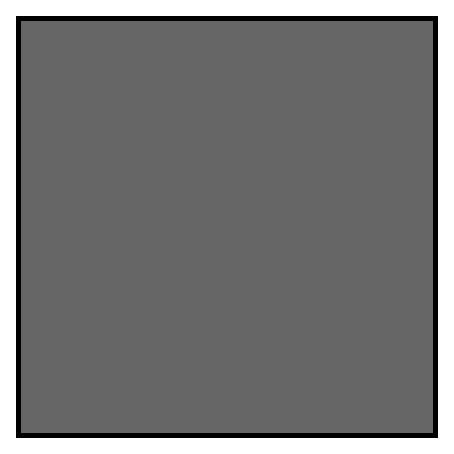
\includegraphics{example.eps}
% figure caption is below the figure
\caption{Please write your figure caption here}
\label{fig:1}       % Give a unique label
\end{figure}
%
% For two-column wide figures use
\begin{figure*}
% Use the relevant command to insert your figure file.
% For example, with the graphicx package use
  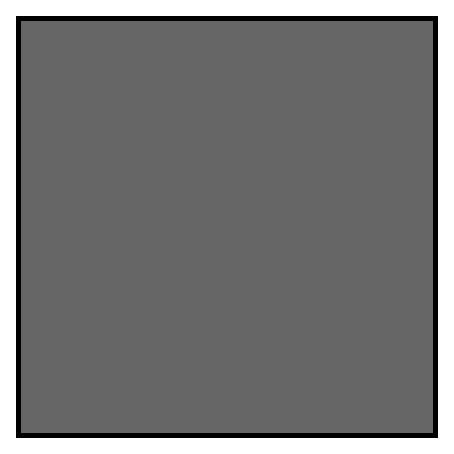
\includegraphics[width=0.75\textwidth]{example.eps}
% figure caption is below the figure
\caption{Please write your figure caption here}
\label{fig:2}       % Give a unique label
\end{figure*}
%
% For tables use
\begin{table}
% table caption is above the table
\caption{Please write your table caption here}
\label{tab:1}       % Give a unique label
% For LaTeX tables use
\begin{tabular}{lll}
\hline\noalign{\smallskip}
first & second & third  \\
\noalign{\smallskip}\hline\noalign{\smallskip}
number & number & number \\
number & number & number \\
\noalign{\smallskip}\hline
\end{tabular}
\end{table}


%\begin{acknowledgements}
%If you'd like to thank anyone, place your comments here
%and remove the percent signs.
%\end{acknowledgements}

% BibTeX users please use one of
%\bibliographystyle{spbasic}      % basic style, author-year citations
%\bibliographystyle{spmpsci}      % mathematics and physical sciences
%\bibliographystyle{spphys}       % APS-like style for physics
%\bibliography{}   % name your BibTeX data base

% Non-BibTeX users please use
\begin{thebibliography}{}
%
% and use \bibitem to create references. Consult the Instructions
% for authors for reference list style.
%
\bibitem{RefJ}
% Format for Journal Reference
Author, Article title, Journal, Volume, page numbers (year)
% Format for books
\bibitem{RefB}
Author, Book title, page numbers. Publisher, place (year)
% etc
\end{thebibliography}

\end{document}
% end of file template.tex